To test the different methods to solve eq.\eqref{eq:wave}. I solved it with parameters $c = 10\;\rm{m/s}$, $L = 10\;\rm{m}$ and $t \in [0, T]$, where $T$ is an arbitrarily chosen constant.
In the implementation I also always choose $\Delta x = L/127$. The time step will be chosen to be $\Delta t = \Delta x/c$.

I solved eq.\eqref{eq:wave} and \eqref{eq:initial} for three different known functions $f(x)$ given as
\begin{eqnarray}
	f(x) & = &e^{-(x-L/2)^2} \label{eq:initNormal}\\
	f(x) & = &sin(0.2 \pi x) \label{eq:initSine}\\
	f(x) & = &\begin{cases}
				1, \qquad L/3 < x < 2 L/3 \\
				0, \qquad else
			\end{cases}\label{eq:initDiscont}
\end{eqnarray}

The solutions are very similar for all methods except for a few exceptions.
When it came to speed and amplitude of the wave, the implicit method (see section \ref{sec:implicit}) damped the solution and also moved slower than the solutions of the other methods, see fig. \ref{fig:normalImplicit} and \ref{fig:normalExplicit}. 

\subsection{Stability with respect to Time Step}
The \emph{explicit} methods, which include the simeple explicit method and the FFT time step method, are unstable for time steps above the \emph{Courant-Lewy-Friedrich} condition (CLF-condition)
where the time step is set to $\Delta t = \Delta x/c$. Smaller time-steps give better results, especially for discontinuous initial function. Which is to be expected.

The \emph{implicit} methods which include the fully implicit method and the Crank-Nicholson method
are stable for any time step. However a higher time step means higher damping. which according to \cite{FDNotes} is to be expected.

%----------------------------------------
%----------------------------------------
%What is the
%maximum dt you 
%an use for the different methods?  (Note, you do not have
%to estimate the exact value of the maximum dt analytically, just discuss it qualitatively.)
%
%Does
%a smaller dt always give a better solution to this problem?
%Can you understand why you 
%annot have
%bigger dt, and why the maximum dt is so different for different methods?
-------------------------------------------


The methods that utilizes the fourier transform handled discontinuous initial functions like eq.\eqref{eq:initDiscont} much better than the other methods, see fig. \ref{fig:discontExplicit} and \ref{fig:discontFFTimmediate}.

\begin{figure}[htbp]
	\centering
	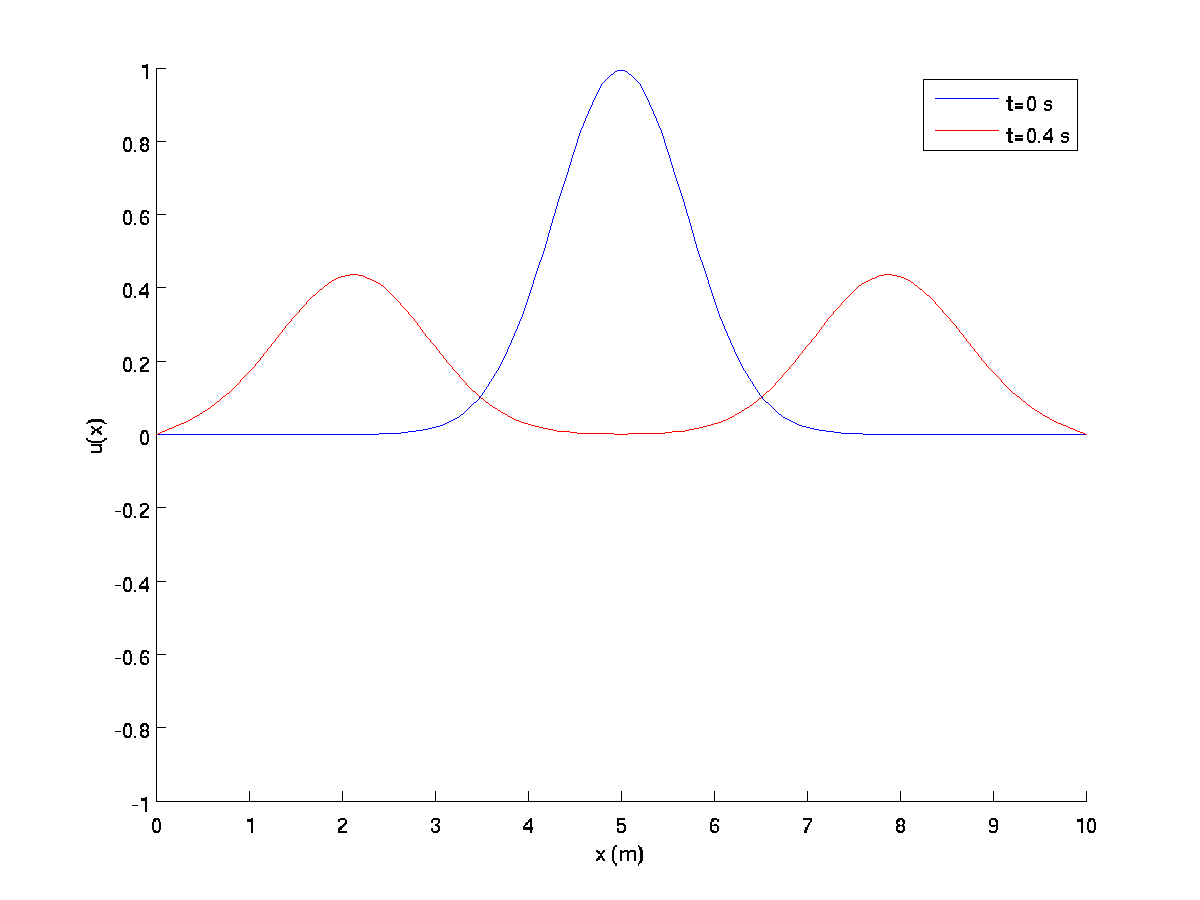
\includegraphics[width=0.8\textwidth]{img/normalImplicit}
	\caption{The solution of the wave equation for a normal initial function using an explicit method.}
	\label{fig:normalImplicit}
\end{figure}

\begin{figure}[htbp]
	\centering
	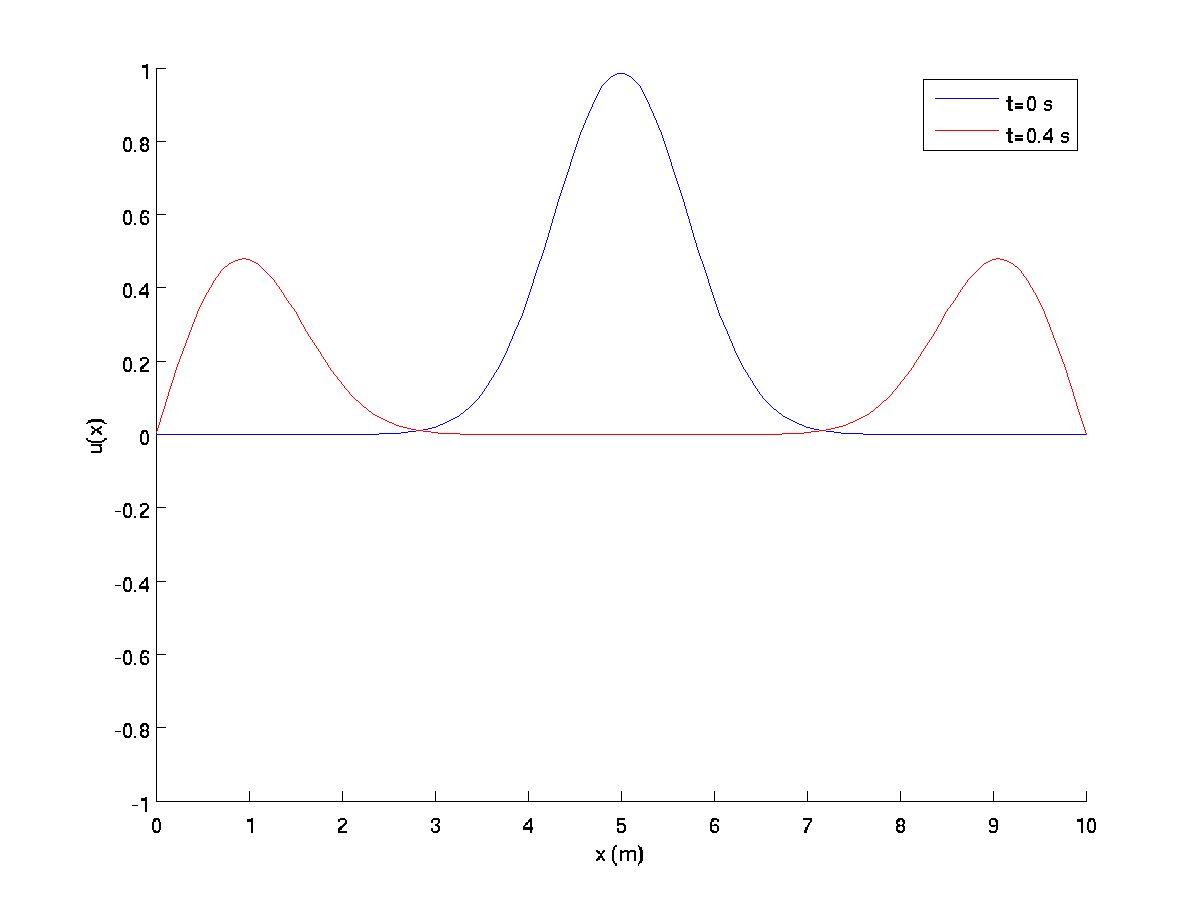
\includegraphics[width=0.8\textwidth]{img/normalExplicit}
	\caption{The solution of the wave equation for a normal initial function using an implicit method.}
	\label{fig:normalExplicit}
\end{figure}

\begin{figure}[htbp]
	\centering
	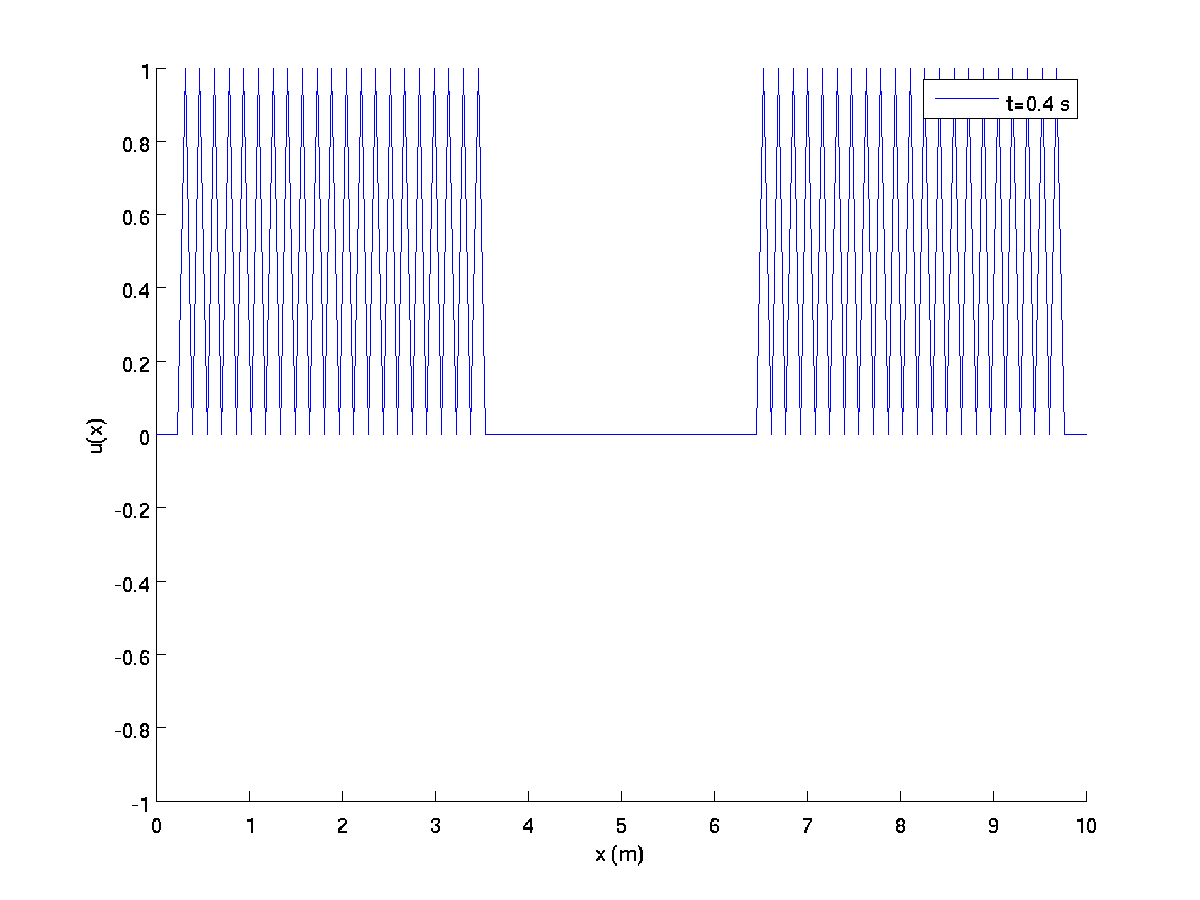
\includegraphics[width=0.8\textwidth]{img/discontExplicit}
	\caption{The solution of the wave equation for a discontinuous initial function using an explicit method.}
	\label{fig:discontExplicit}
\end{figure}

\begin{figure}[htbp]
	\centering
	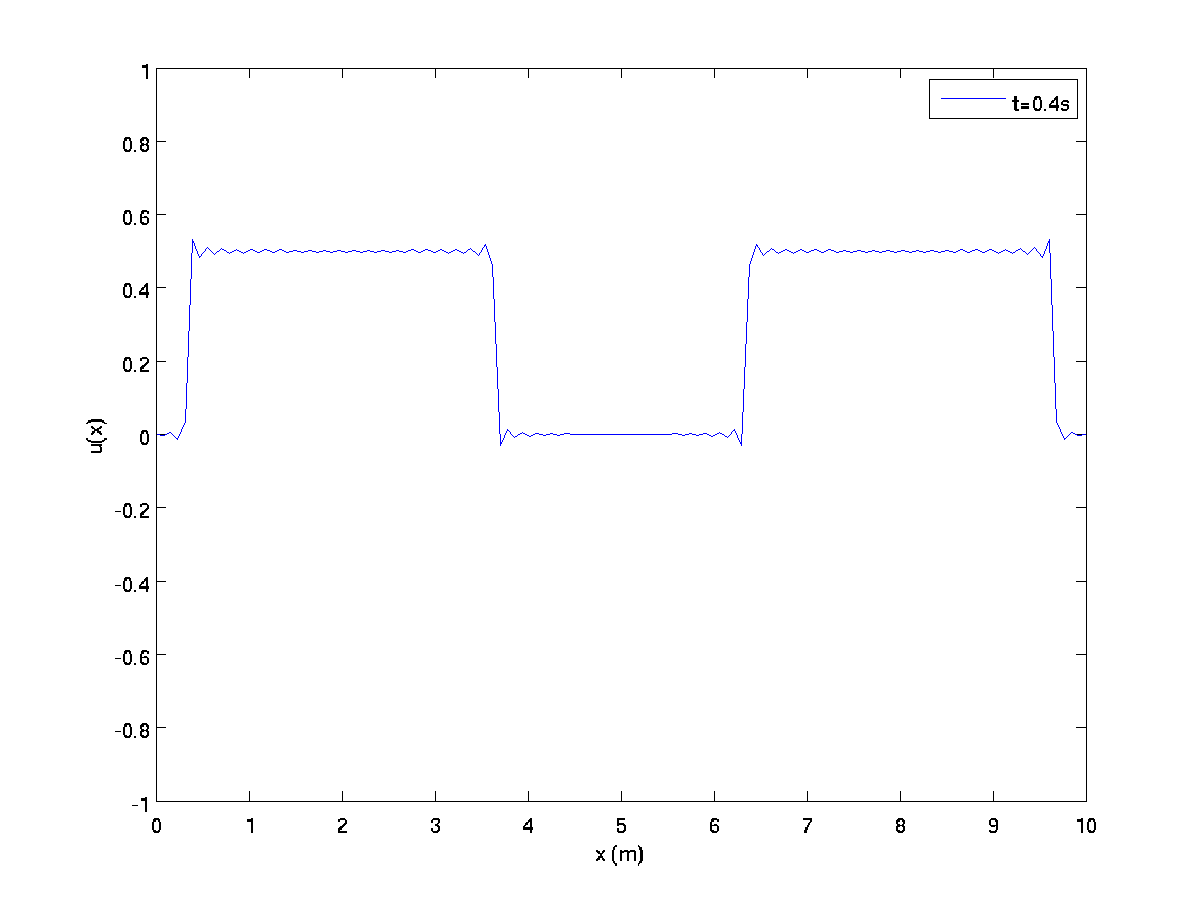
\includegraphics[width=0.8\textwidth]{img/discontFFTimmediate}
	\caption{The solution of the wave equation for a discontinuous initial function using the fourier transform method without time-step.}
	\label{fig:discontFFTimmediate}
\end{figure}


